\documentclass[11pt]{article}
% ---------------------------------------------------------------------------
% Reading the Book -- subscription signals and the IPO pop. pdfLaTeX + BibTeX (Overleaf default).
% tables/ and figures/ are generated by make_paper3.py from ../data/signals.json and ../data/pm.json.
% ---------------------------------------------------------------------------
\usepackage[T1]{fontenc}
\usepackage[utf8]{inputenc}
\usepackage{mathpazo}
\usepackage[scaled=0.92]{helvet}
\usepackage{microtype}
\usepackage[a4paper,margin=2.4cm]{geometry}
\usepackage{amsmath,amssymb}
\usepackage{booktabs,threeparttable,array,tabularx}
\usepackage{graphicx}
\usepackage[font=small,labelfont=bf,labelsep=period,skip=4pt]{caption}
\usepackage{xcolor}
\usepackage{enumitem}
\usepackage[round,authoryear]{natbib}
\usepackage{fancyhdr}
\usepackage{titlesec}
\usepackage[colorlinks=true,linkcolor=accent,citecolor=accent,urlcolor=accent]{hyperref}

\definecolor{accent}{HTML}{1C5CAB}
\definecolor{muted}{HTML}{52514E}
\titleformat{\section}{\normalfont\large\bfseries\color{accent}}{\thesection}{0.8em}{}
\titleformat{\subsection}{\normalfont\normalsize\bfseries}{\thesubsection}{0.8em}{}
\setlength{\parskip}{0.35em}
\setlist{itemsep=0.2em,topsep=0.3em}
\renewcommand{\arraystretch}{1.12}
\newcolumntype{Y}{>{\raggedright\arraybackslash}X}
\pagestyle{fancy}\fancyhf{}
\fancyhead[L]{\small\color{muted}Reading the book: subscription signals and the IPO pop}
\fancyhead[R]{\small\color{muted}15 November 2026}
\fancyfoot[C]{\small\thepage}
\renewcommand{\headrulewidth}{0.4pt}

\title{\vspace{-1.2em}\textbf{Reading the Book}\\[0.3em]
\large Subscription Signals, the First-Day Pop and What Follows,\\ Intraday and Close to Close, with Prediction-Market Context for Anthropic}
\author{CrossAssetMacro Research}
\date{15 November 2026\\[0.2em]\small Market data to 13 November 2026}

\begin{document}
\maketitle
\thispagestyle{fancy}

\begin{abstract}
\noindent Does the order book tell you how a new stock will trade? We take 43 large US IPOs since September 2020 and line up what was knowable before the first trade (the price revision against the first filed range, whether the range was raised, upsizing, reported oversubscription, float, deal size and crowding in speculative assets) against every part of the debut: the opening print, the drift from open to close, the close against the intraday high, the day-2 gap, and returns to day 5, 21 and 63. The answer is sharp. \textbf{Book-building demand sets the opening print and nothing after it.} The price revision has a rank correlation of 0.76 with the opening pop and explains about half of its variation; it has no relation to the open-to-close move ($\rho=-0.04$, $R^2=0.02$ for all signals together) or to returns over the next five days. The opening print is 107\% of the average log first-day return: once trading starts, the stock drifts slightly lower. Hot deals (range raised, priced above it; median opening pop $+55\%$) close nearly 10\% below their intraday high and are the only group that fades by day 63 ($-20\%$, $-27\%$ against Nasdaq-100). Cold deals broke issue 43\% of the time. Headline oversubscription multiples, which dominate press coverage, are uninformative or inverse in our seven reported cases. The money is in the allocation, not the aftermarket: subscribing to hot deals returned a mean $+65\%$ at the first close with a 95\% hit rate, while buying the opening print lost money on average at every horizon from the close to day 63. For Anthropic, which prices on 18 November after a book reported at about six times covered by the third roadshow day, a signal model calibrated on the cohort implies a $+22\%$ first-day return at the prediction-market offer of about \$88 (80\% range $-4\%$ to $+50\%$); Polymarket's median is $+31\%$. Both say the same thing about where to be: in the allocation, out of the open.
\end{abstract}

\section*{Key findings}
\begin{enumerate}[leftmargin=1.4em]
\item \textbf{Demand prices the open, then stops.} Price revision vs opening pop: $\rho=0.76$ ($q<0.05$). Vs open-to-close: $\rho=-0.04$. Vs day 1 to 5: $\rho=-0.01$. All information in the book is in the first print (Tables~\ref{tab:s2}, \ref{tab:s3}).
\item \textbf{The opening print overshoots the day.} Summed across IPOs, the open accounts for 107\% of the log first-day return. Median open-to-close is negative in every demand group ($-0.8\%$ cold, $-4.6\%$ warm, $-2.8\%$ hot).
\item \textbf{Hotter books leave longer upper wicks.} Price revision vs close-relative-to-high: $\rho=-0.35$. Hot deals close a median 9.8\% below their day-1 high; cold deals 5.4\%.
\item \textbf{Close to close, groups do not differ for a month.} Day-2 gap, day 1--5 and day 1--21 returns are flat across groups (Kruskal--Wallis $p\ge0.78$). By day 63 hot deals lag ($-20\%$ median) and cold deals lead ($+14\%$); crowding at listing, not book demand, predicts that fade ($\rho=-0.37$).
\item \textbf{Cold books break.} 71\% of IPOs priced at or below the first-range midpoint closed day 1 below the offer; none of the 15 priced more than 20\% above it did.
\item \textbf{Oversubscription headlines mislead.} Among seven deals with reported coverage, more coverage meant a lower pop ($\rho=-0.70$, $p=0.08$); the three 20$\times$ books all sold off after the open.
\item \textbf{Subscribe; do not chase.} Mean return at the first close: subscribing $+37\%$ (all), $+65\%$ (hot); buying the open $-1\%$. Buying the open of a hot deal and holding 63 days lost $7\%$ on average with a 30\% hit rate (Table~\ref{tab:s8}).
\item \textbf{Anthropic.} Model $+22\%$ pop at the market-implied \$88 offer, $+7\%$ at the \$74 midpoint; Polymarket $+31\%$ median, 90\% probability of closing above the offer. Anthropic's crowding reading is the lowest in the sample and its size is unprecedented, so the model extrapolates on both.
\end{enumerate}

\section{Question and design}
The IPO literature has known since \citet{hanley1993} that the revision from the filed range to the offer predicts underpricing: bankers only partially adjust the price to strong demand, so information revealed in the book spills into the first-day return. Partial adjustment is a statement about the first close. Traders care about more than that: whether the information lands at the opening print or during the day, whether the stock keeps going after day 1, and whether it is better to be allocated, to buy the open or to wait. This paper decomposes the debut into its parts and asks which pre-trade signals predict which part.

\paragraph{Sample.} 43 US IPOs from September 2020 (Snowflake) to June 2026 (SpaceX), all raising at least \$500m or valued above \$5bn at listing; the cohort of the companion paper \citep{frenzyfade2026}. 42 had a filed price range; SpaceX priced at a fixed \$135 and is excluded from range-based signals. Prices are daily and 60-minute bars from Yahoo Finance; hourly debut data are available for 14 IPOs since 2024.

\paragraph{Signals} (all known before the first trade; Table~\ref{tab:s1}):
\begin{itemize}[leftmargin=1.2em]
\item \textit{Price revision}: offer price against the midpoint of the first filed range, the \citet{hanley1993} measure.
\item \textit{Range revision}: final range midpoint against the first; \textit{offer vs final range}; indicators for pricing above the first range and for a range raised before pricing.
\item \textit{Upsized}: more shares sold than first filed. \textit{Float}: shares sold over shares outstanding. \textit{Deal size}: log proceeds.
\item \textit{Reported oversubscription}: book coverage in roadshow press reports, available for seven IPOs.
\item \textit{Crowding at listing} (CROWD) and \textit{positioning} (PSI): composites of high-beta, momentum, Bitcoin, IPO-ETF and sector momentum, and low realised volatility, measured the day before listing, from the companion paper.
\end{itemize}
We group deals three ways by demand: \textit{cold} (priced at or below the first range, $n=14$), \textit{warm} (priced above the first range without raising it, $n=8$) and \textit{hot} (range raised and priced above it, $n=20$). A second grouping uses the size of the price revision.

\paragraph{Outcomes.} Opening pop (first print vs offer); open to close on day 1; close vs intraday high; first-day return or ``pop'' (close vs offer); day-2 gap (day-2 open vs day-1 close); and returns from the first close to day 5, 21 and 63, raw and against QQQ. Inference uses Spearman correlations with Benjamini--Hochberg $q$-values \citep{benjamini1995}, Kruskal--Wallis tests across groups and OLS with HC3 errors.

\begin{table}[!htbp]\centering\footnotesize
\caption{Book-building signals in the cohort}\label{tab:s1}

\begin{threeparttable}
\begin{tabular}{lrrrr}
\toprule
Signal & $n$ & Mean & Median & Range \\
\midrule
Price revision (offer vs first-range midpoint) & 42 & +14.3 & +11.4 & $-$42 to +56 \\
Range revision (final vs first midpoint) & 42 & +6.8 & 0.0 & $-$42 to +39 \\
Offer vs final-range midpoint & 42 & +6.6 & +6.8 & $-$22 to +19 \\
Priced above first range (share) & 42 & 67\% & -- & -- \\
Range raised before pricing (share) & 42 & 48\% & -- & -- \\
Upsized (share) & 43 & 35\% & -- & -- \\
Reported oversubscription (times) & 7 & 13.2$\times$ & 19$\times$ & 3.5$\times$ to 20$\times$ \\
\bottomrule
\end{tabular}
\begin{tablenotes}[flushleft]\footnotesize
\item \textit{Notes:} Percent unless stated. Ranges and offer prices from SEC 424B4 prospectuses and pricing releases; upsizing and oversubscription from pricing releases and Reuters, Bloomberg and CNBC reports. SpaceX priced at a fixed \$135 with no range and is excluded from range-based signals.
\end{tablenotes}
\end{threeparttable}

\end{table}


\section{Which signal predicts which part of the debut}
Table~\ref{tab:s2} is the core result. Read across the first row: the price revision correlates 0.76 with the opening pop and 0.67 with the first-day return, but $-0.04$ with the open-to-close move, $-0.01$ with days 1--5 and $-0.15$ with days 1--63. Every revision-type signal shows the same pattern: strong for the opening print, nothing for the session or the week after. Upsizing, float and deal size predict none of the debut. Crowding and positioning at listing raise the open a little and are the only signals that predict the three-month fade, which is the companion paper's result reappearing here.

\begin{table}[!htbp]\centering\footnotesize
\caption{Which signals predict which part of the debut? Rank correlations}\label{tab:s2}
\resizebox{\linewidth}{!}{
\begin{threeparttable}
\begin{tabular}{lrrrrrrr}
\toprule
Signal & Open vs offer & Open$\to$close & Close vs high & Close vs offer & Day-2 gap & D1$\to$D5 & D1$\to$D63 \\
\midrule
Price revision & 0.76$^{\dagger}$ & $-$0.04 & $-$0.35$^{*}$ & 0.67$^{\dagger}$ & 0.20 & $-$0.01 & $-$0.15 \\
Range revision & 0.65$^{\dagger}$ & $-$0.04 & $-$0.39$^{*}$ & 0.55$^{\dagger}$ & 0.23 & $-$0.03 & $-$0.09 \\
Offer vs final range & 0.71$^{\dagger}$ & 0.04 & $-$0.20 & 0.66$^{\dagger}$ & 0.12 & 0.04 & $-$0.06 \\
Above first range & 0.60$^{\dagger}$ & $-$0.13 & $-$0.21 & 0.50$^{\dagger}$ & 0.18 & $-$0.01 & $-$0.25 \\
Range raised & 0.63$^{\dagger}$ & $-$0.01 & $-$0.31 & 0.53$^{\dagger}$ & 0.20 & $-$0.09 & $-$0.15 \\
Upsized & $-$0.04 & 0.19 & 0.37$^{*}$ & 0.05 & 0.00 & 0.37$^{*}$ & 0.06 \\
Float & $-$0.15 & 0.06 & 0.24 & $-$0.08 & 0.07 & 0.28 & 0.13 \\
log proceeds & $-$0.07 & 0.20 & 0.13 & 0.07 & $-$0.06 & 0.18 & 0.04 \\
Crowding at listing & 0.50$^{\dagger}$ & $-$0.01 & $-$0.37$^{*}$ & 0.44$^{\dagger}$ & 0.11 & $-$0.13 & $-$0.37$^{*}$ \\
Positioning (PSI) & 0.42$^{\dagger}$ & $-$0.10 & $-$0.25 & 0.37$^{*}$ & 0.26 & $-$0.25 & $-$0.51$^{\dagger}$ \\
\bottomrule
\end{tabular}
\begin{tablenotes}[flushleft]\footnotesize
\item \textit{Notes:} Spearman $\rho$, 42--43 IPOs. $^{\dagger}q<0.05$, $^{*}q<0.10$ (Benjamini--Hochberg over all signal--outcome pairs). Close vs offer is the first-day return (``pop''); later returns are measured from the first close.
\end{tablenotes}
\end{threeparttable}
}
\end{table}


Table~\ref{tab:s3} turns this into a decomposition. Writing the log first-day return as the log opening pop plus the log open-to-close return, the price revision carries a coefficient of 0.69 on the first part ($t=3.4$, $R^2=0.48$) and $-0.01$ on the second ($R^2=0.02$ for all three signals). The book's information is incorporated before the first trade, through the auction that sets the opening print. What happens next is noise with a slight negative drift.

\begin{table}[!htbp]\centering\footnotesize
\caption{Demand prices the open; nothing prices the rest of the day}\label{tab:s3}

\begin{threeparttable}
\begin{tabular}{lrrrrr}
\toprule
Dependent variable & Price revision & Crowding & log proceeds & $R^2$ & $n$ \\
\midrule
log(1+opening pop) & 0.69 (3.4) & 0.11 (1.9) & 0.00 ($-$0.1) & 0.48 & 42 \\
log(1+open$\to$close) & $-$0.01 ($-$0.2) & 0.00 (0.0) & 0.02 (0.8) & 0.02 & 42 \\
log(1+first-day return) & 0.68 (2.8) & 0.11 (1.6) & 0.02 (0.3) & 0.35 & 42 \\
Day 1$\to$5 & 0.13 (0.6) & $-$0.13 ($-$1.6) & 0.08 (1.3) & 0.15 & 42 \\
Day 1$\to$63 & $-$0.02 (0.0) & $-$0.32 ($-$2.3) & 0.05 (0.5) & 0.12 & 42 \\
\bottomrule
\end{tabular}
\begin{tablenotes}[flushleft]\footnotesize
\item \textit{Notes:} OLS with HC3 $t$-statistics. Across the cohort the opening print accounts for 107\% of the summed log first-day return: on average the stock drifts slightly lower after it opens.
\end{tablenotes}
\end{threeparttable}

\end{table}


\begin{figure}[!htbp]\centering
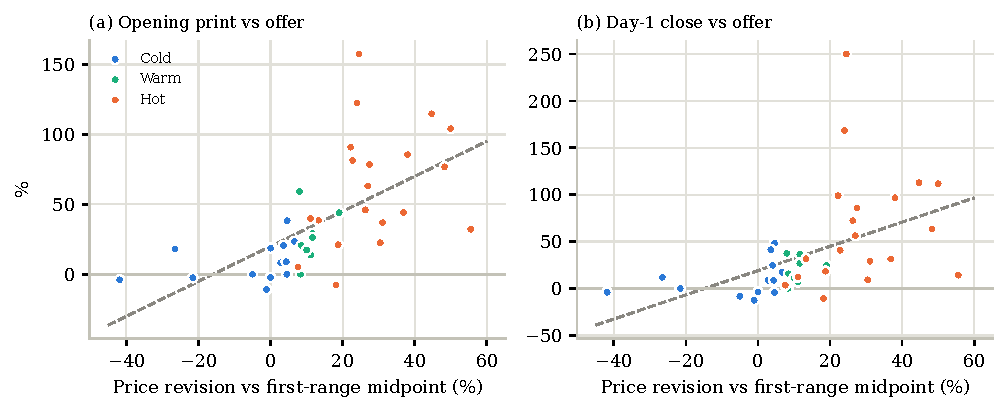
\includegraphics[width=\linewidth]{figures/f1_rev}
\caption{Price revision against the opening pop (a) and the first-day return (b). Colour = book-building group; dashed line = OLS fit. The slope is almost the same in both panels: the book's information arrives at the opening print, and the rest of the session neither adds to it nor takes it away on average.}\label{fig:rev}
\end{figure}

\section{Intraday: the opening print overshoots}
Table~\ref{tab:s4} and Figure~\ref{fig:anatomy} show the debut by demand group. The opening pop rises steeply with demand: $+9\%$ cold, $+23\%$ warm, $+55\%$ hot (Kruskal--Wallis $p<0.001$). The move from open to close is negative in all three groups and not different between them ($p=0.58$). Hot deals trade further above where they close: the median hot IPO closes 9.8\% below its day-1 high against 5.4\% for cold deals, and the price revision correlates $-0.35$ with close-vs-high. The intraday high is set early: the opening auction concentrates demand that the book could not fill, and the session absorbs flipping by allocated investors.

\begin{table}[!htbp]\centering\scriptsize
\caption{Debut and aftermarket by book-building signal}\label{tab:s4}
\resizebox{\linewidth}{!}{
\begin{threeparttable}
\begin{tabular}{lrrrrrrrrrrr}
\toprule
Group & $n$ & Open & Open$\to$close & Close vs high & Pop & Broke & Day-2 gap & D1$\to$5 & D1$\to$21 & D1$\to$63 & D63 vs QQQ \\
\midrule
Cold: at or below first range & 14 & +9 & $-$0.8 & $-$5.4 & +4 & 43\% & 0.0 & +5.3 & +0.5 & +14 & +8 \\
Warm: above first range & 8 & +23 & $-$4.6 & $-$6.4 & +20 & 0\% & $-$0.1 & +6.5 & $-$0.5 & $-$16 & $-$23 \\
Hot: range raised and priced above it & 20 & +55 & $-$2.8 & $-$9.8 & +48 & 5\% & +2.3 & +1.9 & $-$2.9 & $-$20 & $-$27 \\
\midrule
Kruskal--Wallis $p$ & & $<$0.001 & 0.58 & & 0.001 & & & 0.78 & 0.86 & 0.27 & \\
\bottomrule
\end{tabular}
\begin{tablenotes}[flushleft]\footnotesize
\item \textit{Notes:} Medians in percent. Broke = share closing day 1 below the offer. Day-2 gap = day-2 open vs day-1 close. Later returns from the first close.
\end{tablenotes}
\end{threeparttable}
}
\end{table}


\begin{figure}[!htbp]\centering
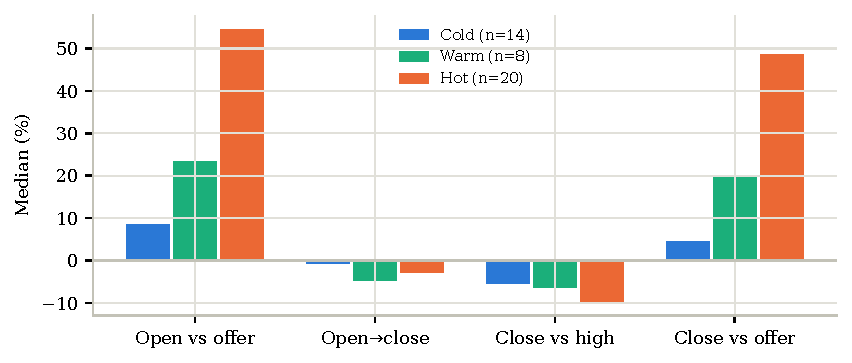
\includegraphics[width=0.92\linewidth]{figures/f2_anatomy}
\caption{Anatomy of the debut by demand group, medians. The opening print carries the whole demand gradient; open-to-close is negative for every group and hot deals close furthest below their high.}\label{fig:anatomy}
\end{figure}

Table~\ref{tab:s5} groups by the size of the price revision instead and makes the tails clearer. Of the seven IPOs priced at or below the first-range midpoint, five (71\%) closed day 1 below the offer: a weak book is a near-certain break. Of the 15 priced more than 20\% above the midpoint, none broke and the median pop was $+72\%$.

\begin{table}[!htbp]\centering\scriptsize
\caption{Debut and aftermarket by size of price revision}\label{tab:s5}
\resizebox{\linewidth}{!}{
\begin{threeparttable}
\begin{tabular}{lrrrrrrrrrrr}
\toprule
Group & $n$ & Open & Open$\to$close & Close vs high & Pop & Broke & Day-2 gap & D1$\to$5 & D1$\to$21 & D1$\to$63 & D63 vs QQQ \\
\midrule
At or below first-range midpoint & 7 & $-$2 & $-$2.0 & $-$5.4 & $-$4 & 71\% & 0.0 & $-$2.3 & $-$0.1 & +14 & +8 \\
Up to 20\% above & 20 & +21 & $-$2.8 & $-$6.0 & +17 & 10\% & +0.4 & +5.2 & $-$1.1 & $-$2 & $-$11 \\
More than 20\% above & 15 & +78 & $-$0.9 & $-$11.7 & +72 & 0\% & +4.7 & $-$4.6 & $-$1.5 & $-$23 & $-$28 \\
\midrule
Kruskal--Wallis $p$ & & $<$0.001 & 0.71 & & $<$0.001 & & & 0.87 & 0.91 & 0.56 & \\
\bottomrule
\end{tabular}
\begin{tablenotes}[flushleft]\footnotesize
\item \textit{Notes:} Medians in percent. Broke = share closing day 1 below the offer. Day-2 gap = day-2 open vs day-1 close. Later returns from the first close.
\end{tablenotes}
\end{threeparttable}
}
\end{table}


Figure~\ref{fig:hourly} uses the 14 debuts with hourly data. It is illustrative rather than conclusive: only four of them are hot deals. In those four, the stock kept rising through the first session and into the second, then gave back about half of the gain in a single hour; the other ten drifted lower for the first two sessions and recovered in the third. The pattern is consistent with the daily evidence that hot debuts have the highest intraday highs relative to their close.

\begin{figure}[!htbp]\centering
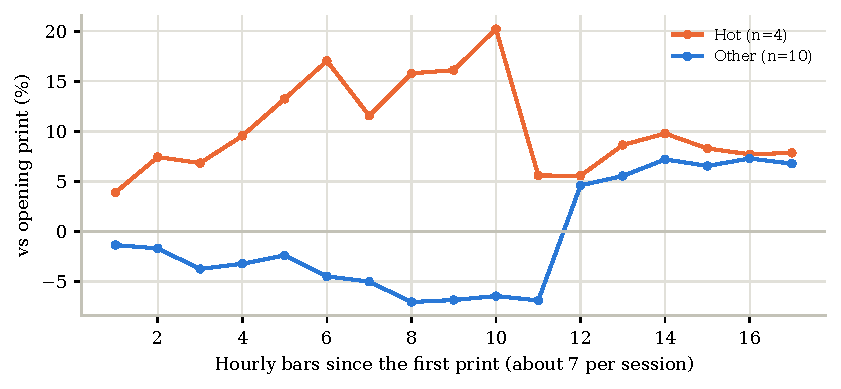
\includegraphics[width=0.85\linewidth]{figures/f3_hourly}
\caption{Median path of 60-minute closes against the opening print, first 2--3 sessions, IPOs listed since 2024 with hourly data. Hot = range raised and priced above it (CoreWeave was cold; Figma, Netskope, Circle and Gemini hot). Small samples.}\label{fig:hourly}
\end{figure}

\section{Close to close: no momentum, then a fade}
After the first close, demand stops mattering for a month. The day-2 gap is a median $+2.3\%$ for hot deals and zero for the others, but the difference is not significant. Returns from the first close to day 5 and to day 21 are statistically the same across groups (Kruskal--Wallis $p=0.78$ and $0.86$). Figure~\ref{fig:c2c} shows the mean cumulative path over the first ten sessions: all three groups drift up a few percent with no ordering by demand.

\begin{figure}[!htbp]\centering
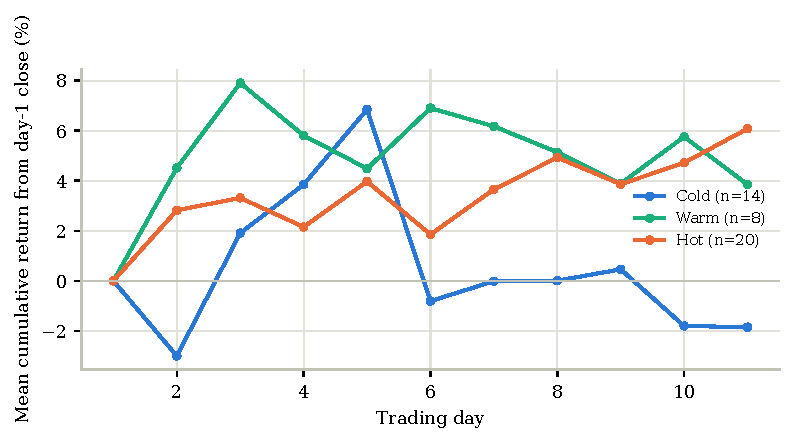
\includegraphics[width=0.8\linewidth]{figures/f4_c2c}
\caption{Mean cumulative return from the day-1 close, trading days 1--11, by demand group. No group shows the momentum a hot book might suggest; the ordering appears only at three months.}\label{fig:c2c}
\end{figure}

By day 63 the ordering emerges and it is inverted: cold deals $+14\%$, warm $-16\%$, hot $-20\%$ (medians; $-27\%$ against QQQ for hot deals). The group difference is not significant on its own ($p=0.27$), and the regression in Table~\ref{tab:s3} attributes the fade to crowding at listing ($t=-2.3$) rather than to the book (coefficient $-0.02$). Hot books and crowded markets tend to coincide; it is the crowding that predicts the fade.

\section{Headline oversubscription}
Coverage multiples (``20 times oversubscribed'') are the most quoted book-building statistic and the least useful. Table~\ref{tab:s6} lists the seven cohort IPOs with reported coverage. The three with 20$\times$ books (Gemini, StubHub, Netskope) all opened up and then sold off during the session; Klaviyo at 19$\times$ did the same. The three with modest coverage (SpaceX 3.5$\times$, Reddit 4$\times$, Arm 6$\times$) all rose from open to close. Rank correlations with coverage: $+0.19$ for the opening pop, $-0.74$ for open-to-close, $-0.70$ for the pop ($p=0.08$), $-0.78$ for day 1--63.

Seven deals cannot establish an inverse relationship, but the mechanism is plausible: coverage is reported on gross orders, which are inflated in anticipation of scaling back when a deal is known to be hot, so a high multiple measures order padding as much as demand \citep{cornelli2006}. The price revision is the better signal because it is what the bankers did with the book, not what they said about it.

\begin{table}[!htbp]\centering\footnotesize
\caption{Headline oversubscription and the debut (7 IPOs with reported book coverage)}\label{tab:s6}
\resizebox{\linewidth}{!}{
\begin{threeparttable}
\begin{tabular}{lrrrrrr}
\toprule
IPO & Book covered & Price revision & Open & Open$\to$close & Pop & D1$\to$D63 \\
\midrule
SpaceX & 3.5$\times$ & -- & +11 & +7 & +19 & $-$6 \\
Reddit & 4$\times$ & +5 & +38 & +7 & +48 & +14 \\
Arm & 6$\times$ & +4 & +10 & +13 & +25 & +2 \\
Klaviyo & 19$\times$ & +30 & +22 & $-$11 & +9 & $-$14 \\
Gemini & 20$\times$ & +56 & +32 & $-$14 & +14 & $-$65 \\
StubHub & 20$\times$ & 0 & +19 & $-$21 & $-$6 & $-$36 \\
Netskope & 20$\times$ & +19 & +21 & $-$2 & +18 & $-$11 \\
\midrule
Spearman $\rho$ with oversubscription & & & 0.19 & $-$0.74 & $-$0.70 ($p=0.08$) & $-$0.78 \\
\bottomrule
\end{tabular}
\begin{tablenotes}[flushleft]\footnotesize
\item \textit{Notes:} Percent. Book coverage as reported during the roadshow (Reuters, Bloomberg), lower bound when reported as a range. The 20$\times$ books all traded lower from open to close; headline coverage is a weak and, if anything, inverse signal for the pop.
\end{tablenotes}
\end{threeparttable}
}
\end{table}

\begin{table}[!htbp]\centering\footnotesize
\caption{Roadshow demand: Anthropic and SpaceX}\label{tab:s7}
\resizebox{\linewidth}{!}{
\begin{threeparttable}
\begin{tabular}{llp{2.7cm}p{3.6cm}p{4.2cm}}
\toprule
IPO & Launch & Terms & Reported book & Notes \\
\midrule
Anthropic & 10 Nov & \$70--78, 825m shares & $\sim$2$\times$ after day 1; $\sim$6$\times$ after day 3 (12 Nov) & Range unchanged as of 15 Nov; concurrent private placement $\sim$\$26bn \\
SpaceX & 2 Jun & Fixed \$135, 556m shares & 2$\times$ after day 2; 3.5--4$\times$ near pricing & Pop $+$19\%; peak day 3; below offer by day 23 \\
\bottomrule
\end{tabular}
\begin{tablenotes}[flushleft]\footnotesize
\item \textit{Notes:} Reuters and Bloomberg reports of 9 June 2026 (SpaceX) and 12--14 November 2026 (Anthropic). Book coverage figures are banker estimates during the roadshow and can change.
\end{tablenotes}
\end{threeparttable}
}
\end{table}


Table~\ref{tab:s7} sets Anthropic's roadshow against SpaceX's. Anthropic's book was reported at about 2$\times$ after its first day and about 6$\times$ by the third, faster than SpaceX (2$\times$ after two days, 3.5--4$\times$ near pricing). The range had not been raised as of 15 November. Anthropic also arranged a concurrent private placement of about \$26bn, which takes demand out of the book and makes the coverage multiple a less direct read of public demand.

\section{When to subscribe, when to buy, when to sell}
Table~\ref{tab:s8} and Figure~\ref{fig:matrix} compare three entry points (allocated at the offer, buying the opening print, buying the day-1 close) and five exits. Three results stand out.
\begin{enumerate}[leftmargin=1.4em]
\item \textbf{The allocation is the trade.} Subscribing returned a mean $+37\%$ at the first close across all IPOs (79\% hit rate) and $+65\%$ in hot deals (95\% hit, per-trade Sharpe 1.0). The return is set at the open: selling at the opening print gave the same mean.
\item \textbf{The aftermarket pays nothing.} Buying the open lost a mean 1.1\% by the close and earned 2--4\% to day 5--63, with hit rates below 50\% and per-trade Sharpe ratios of 0.0--0.2. Buying the day-1 close is no better.
\item \textbf{Hot deals are the worst aftermarket buys at three months.} Buying a hot deal's open and holding to day 63 lost a mean 7\% with a 30\% hit rate. Cold deals were the best aftermarket buys ($+25\%$ mean, 71\% hit), but that average depends on a few large winners from 2020--21.
\end{enumerate}
The subscription returns assume full allocation at the offer. In hot deals retail and smaller institutions are heavily scaled back, so the realised return on capital committed is a fraction of the table's figures \citep{aggarwal2002}.

\begin{table*}[!htbp]\centering\scriptsize
\caption{When to subscribe, when to buy, when to sell: mean return / hit rate / Sharpe per trade}\label{tab:s8}
\resizebox{\linewidth}{!}{
\begin{threeparttable}
\begin{tabular}{llllll}
\toprule
Entry & Exit at open & Day-1 close & Day 5 & Day 21 & Day 63 \\
\midrule
\multicolumn{6}{l}{\textit{All} ($n=43$)} \\
\quad Subscribe at offer & +37.3 / 81 / 0.95 & +37.1 / 79 / 0.72 & +42.9 / 84 / 0.74 & +44.0 / 81 / 0.47 & +38.0 / 67 / 0.47 \\
\quad Buy the open & -- & $-$1.1 / 35 / $-$0.10 & +4.2 / 49 / 0.16 & +1.9 / 44 / 0.05 & +2.1 / 44 / 0.03 \\
\quad Buy the day-1 close & -- & -- & +5.3 / 58 / 0.22 & +2.5 / 47 / 0.08 & +2.7 / 42 / 0.05 \\
\multicolumn{6}{l}{\textit{Cold: at or below first range} ($n=14$)} \\
\quad Subscribe at offer & +9.0 / 57 / 0.67 & +8.7 / 50 / 0.47 & +15.2 / 64 / 0.45 & +6.7 / 64 / 0.28 & +34.9 / 71 / 0.40 \\
\quad Buy the open & -- & $-$0.5 / 36 / $-$0.05 & +6.0 / 50 / 0.20 & $-$2.1 / 50 / $-$0.11 & +25.4 / 71 / 0.29 \\
\quad Buy the day-1 close & -- & -- & +6.9 / 57 / 0.21 & $-$1.5 / 50 / $-$0.08 & +24.7 / 71 / 0.29 \\
\multicolumn{6}{l}{\textit{Warm: above first range} ($n=8$)} \\
\quad Subscribe at offer & +26.3 / 88 / 1.43 & +19.9 / 88 / 1.45 & +24.5 / 100 / 1.63 & +25.4 / 100 / 0.89 & +6.0 / 50 / 0.20 \\
\quad Buy the open & -- & $-$4.6 / 25 / $-$0.68 & $-$0.2 / 62 / $-$0.01 & +0.1 / 50 / 0.01 & $-$15.7 / 25 / $-$0.73 \\
\quad Buy the day-1 close & -- & -- & +4.5 / 75 / 0.35 & +5.3 / 50 / 0.23 & $-$11.5 / 25 / $-$0.49 \\
\multicolumn{6}{l}{\textit{Hot: range raised and priced above it} ($n=20$)} \\
\quad Subscribe at offer & +62.7 / 95 / 1.48 & +64.8 / 95 / 1.02 & +70.0 / 90 / 0.98 & +79.6 / 85 / 0.62 & +54.4 / 70 / 0.60 \\
\quad Buy the open & -- & $-$0.7 / 35 / $-$0.05 & +3.7 / 40 / 0.13 & +5.9 / 40 / 0.11 & $-$7.1 / 30 / $-$0.16 \\
\quad Buy the day-1 close & -- & -- & +4.0 / 50 / 0.17 & +5.0 / 45 / 0.13 & $-$6.6 / 30 / $-$0.16 \\
\bottomrule
\end{tabular}
\begin{tablenotes}[flushleft]\footnotesize
\item \textit{Notes:} Each cell: mean return in percent / share of trades that made money / mean divided by standard deviation. Subscribing assumes a full allocation at the offer, which hot deals rarely give. Costs, borrow and allocation size are ignored.
\end{tablenotes}
\end{threeparttable}
}
\end{table*}


\begin{figure}[!htbp]\centering
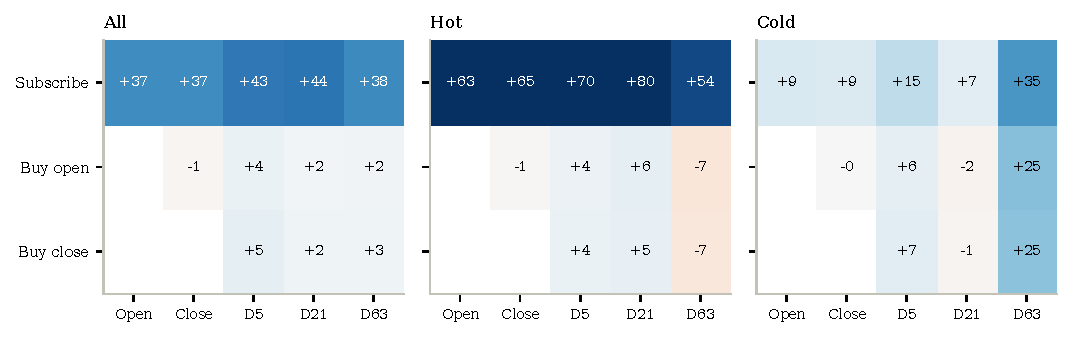
\includegraphics[width=\linewidth]{figures/f5_matrix}
\caption{Mean return (\%) by entry point (rows) and exit (columns), for all IPOs, hot deals and cold deals. The blue band in the top row is the allocation premium; everything below it is close to zero.}\label{fig:matrix}
\end{figure}

\section{Prediction-market context for Anthropic}
Polymarket and Kalshi list markets on Anthropic's IPO date, valuation, amount raised, share of the company sold, lead underwriter, and day-1 closing market cap. The companion paper combines them into an implied distribution for the offer price and the first-day close; Table~\ref{tab:s11} summarises it as of 15 November. Prediction markets expect the deal to price well above the \$70--78 range (about \$85--88; 72--83\% probability of an offer above \$78) and to close day 1 at about \$116, a market cap of about \$1.45tn. The implied median pop is $+31\%$, with a 10th--90th percentile range of $-12\%$ to $+85\%$; the direct ``closes above offer'' market is at 90\%.

\begin{table}[!htbp]\centering\footnotesize
\caption{What prediction markets expect (15 November 2026)}\label{tab:s11}

\begin{threeparttable}
\begin{tabular}{lrrr}
\toprule
Quantity & Mean & Median & 10th--90th percentile \\
\midrule
Day-1 closing market cap (\$tn) & 1.45 & 1.41 & 1.06--1.87 \\
Offer implied by valuation market (\$) & 84.6 & 84.7 & 72.2--95.2 \\
Offer implied by amount-raised market (\$) & 87.9 & 85.7 & 73.2--103.2 \\
Day-1 closing share price (\$) & 116.1 & 112.5 & 80.6--154.2 \\
First-day return (\%) & +35 & +31 & $-$12 to +85 \\
P(offer $>$ \$78): valuation / amount raised & \multicolumn{3}{l}{72\% / 83\%} \\
P(close $>$ offer), P(open $>$ offer), direct markets & \multicolumn{3}{l}{89.5\%, 94\%} \\
Kalshi: IPO before 20 Nov; Goldman Sachs lead-left & \multicolumn{3}{l}{97--98\%; 99\%} \\
\bottomrule
\end{tabular}
\begin{tablenotes}[flushleft]\footnotesize
\item \textit{Notes:} Polymarket bracket markets combined by Monte Carlo; fully diluted shares 18.0bn, basic shares implied by the share-sold market ($\approx$12.6bn), 825 million shares sold. See the companion paper for definitions and the SpaceX calibration.
\end{tablenotes}
\end{threeparttable}

\end{table}


How much should these numbers be trusted? The only comparable test is SpaceX in June 2026 (Table~\ref{tab:s12}). The month-end market cap market placed 41\% on the \$2.0--2.5tn bracket before trading; SpaceX closed day 1 at \$2.17tn, inside that bracket; the expected value moved from \$2.21tn before trading to \$1.95tn after the first session. One observation is a calibration check, not a track record, but the market was well centred.

\begin{table}[!htbp]\centering\footnotesize
\caption{Calibration check: SpaceX end-of-IPO-month market cap (Polymarket)}\label{tab:s12}

\begin{threeparttable}
\begin{tabular}{lrr}
\toprule
Bracket & Before trading & After day 1 \\
\midrule
<\$1.0T & 9\% & 5\% \\
\$1.0-1.5T & 9\% & 13\% \\
\$1.5-2.0T & 13\% & 30\% \\
\$2.0-2.5T & 41\% & 44\% \\
\$2.5-3.0T & 16\% & 7\% \\
\$3.0-3.5T & 4\% & 1\% \\
\$3.5T+ & 7\% & 1\% \\
\midrule
Expected value (\$tn) & 2.21 & 1.95 \\
Outcome & \multicolumn{2}{l}{\$2.0--2.5tn bracket; day-1 close \$2.11tn} \\
\bottomrule
\end{tabular}
\begin{tablenotes}[flushleft]\footnotesize
\item \textit{Notes:} Normalised mid prices at 00:00 UTC on 12 and 13 June 2026.
\end{tablenotes}
\end{threeparttable}

\end{table}


\section{Putting it together: a model of Anthropic's pop}
Table~\ref{tab:s9} fits the log first-day return on the price revision, crowding at listing and deal size. The price revision carries the model ($t=2.8$); in-sample $R^2$ is 0.35 and leave-one-out $R^2$ is 0.23, so out of sample the model explains about a quarter of the variation in pops. Table~\ref{tab:s10} applies it to Anthropic at four offer prices.

\begin{table}[!htbp]\centering\footnotesize
\caption{A model of the first-day return from book-building signals}\label{tab:s9}

\begin{threeparttable}
\begin{tabular}{lrr}
\toprule
Variable & Coefficient & $t$ (HC3) \\
\midrule
Intercept & 0.063 & 0.2 \\
Price revision & 0.676 & 2.8 \\
Crowding at listing & 0.115 & 1.6 \\
log proceeds & 0.015 & 0.3 \\
\midrule
$R^2$ (in sample) / leave-one-out $R^2$ & 0.35 & 0.23 \\
$n$ & 42 & \\
\bottomrule
\end{tabular}
\begin{tablenotes}[flushleft]\footnotesize
\item \textit{Notes:} Dependent variable log(1+first-day return). Leave-one-out $R^2$ refits the model without each IPO and predicts it.
\end{tablenotes}
\end{threeparttable}

\end{table}

\begin{table}[!htbp]\centering\footnotesize
\caption{Anthropic: first-day return implied by the signal model and by prediction markets}\label{tab:s10}
\resizebox{\linewidth}{!}{
\begin{threeparttable}
\begin{tabular}{lrrrrr}
\toprule
Scenario & Offer & Revision & Expected pop & 80\% range & P(close $>$ offer) \\
\midrule
Prediction-market offer (amount raised) & \$87.9 & +19 & +22 & $-$4 to +50 & 81\% \\
Prediction-market offer (valuation) & \$84.6 & +14 & +18 & $-$7 to +45 & 81\% \\
Top of range (\$78) & \$78.0 & +5 & +11 & $-$12 to +37 & 60\% \\
Midpoint of range (\$74) & \$74.0 & 0 & +7 & $-$16 to +32 & 55\% \\
\midrule
Same, prediction-market offer, crowding at the cohort median & \$87.9 & +19 & +42 & -- & -- \\
Prediction markets directly (Polymarket) & \$87.9 & +19 & +31 (median) & $-$12 to +85 & 90\% \\
\bottomrule
\end{tabular}
\begin{tablenotes}[flushleft]\footnotesize
\item \textit{Notes:} Model rows use Anthropic's crowding composite on 13 November (-1.43, below the cohort minimum of -1.13) and proceeds of 825 million shares at the offer, far above any cohort deal; both are extrapolations. Ranges add the model's residuals. The last row is the market-implied distribution of Section~6.
\end{tablenotes}
\end{threeparttable}
}
\end{table}


At the prediction-market offer of about \$88 (a 19\% revision against the \$74 midpoint) the model's expected pop is $+22\%$ with an 80\% range of $-4\%$ to $+50\%$ and an 81\% probability of closing above the offer. At the top of the range it is $+11\%$; at the midpoint $+7\%$, with close to even odds of breaking issue. Polymarket's $+31\%$ median sits between the model at Anthropic's own crowding reading ($+22\%$) and the model with crowding at the cohort median ($+42\%$).

Two features of Anthropic lie outside the sample. Its crowding composite on 13 November was the lowest in the cohort: speculative assets had sold off in the weeks before the deal, which lowers the predicted pop and, on the companion paper's evidence, also lowers the risk of a three-month fade. And at roughly \$60--70bn it would be the largest IPO in the sample by a factor of two or more; deal size has no effect in the cohort, but the cohort contains nothing this large.

\begin{figure}[!htbp]\centering
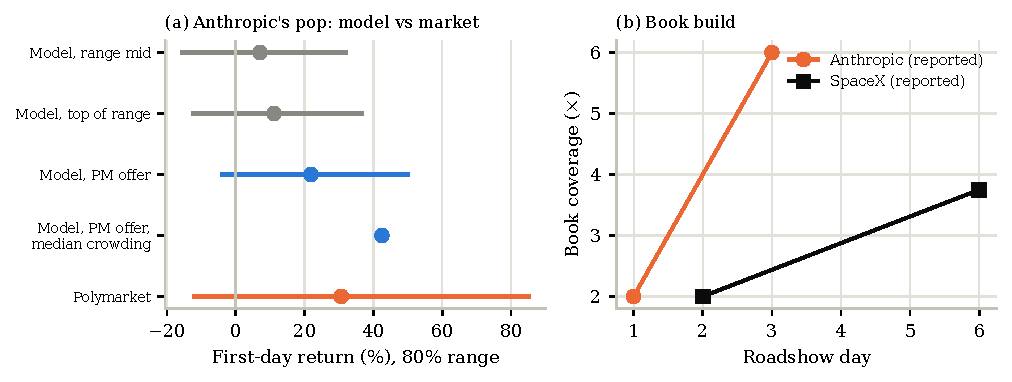
\includegraphics[width=\linewidth]{figures/f6_anthropic}
\caption{(a) Anthropic's first-day return: signal model at four offer assumptions against the Polymarket distribution (dot = expected or median, bar = 10th--90th percentile). (b) Reported book coverage during the roadshow, Anthropic against SpaceX.}\label{fig:ant}
\end{figure}

\section{Hypotheses for the Anthropic debut}
Each hypothesis is stated so that the debut can confirm or reject it.
\begin{description}[leftmargin=1.2em,style=nextline]
\item[H1. The price revision sets the opening print.] If Anthropic prices at \$85--88, the opening pop will be in the $+15\%$ to $+40\%$ band implied by the cohort slope. A revision near zero (offer in the range) predicts an opening pop below $+10\%$ and a real chance of breaking issue.
\item[H2. The open overshoots the close.] The day-1 close will be below the opening print, and further below the intraday high than for a typical deal, if the range is raised before pricing (a hot deal on our definition).
\item[H3. No day-2 to day-5 momentum.] Returns from the first close to day 5 will be within $\pm5\%$; the size of the book will not predict them.
\item[H4. Coverage headlines do not add information.] A final reported coverage above 10$\times$ will not predict a larger pop than the revision already implies.
\item[H5. The fade depends on crowding, not demand.] With crowding at the bottom of the historical range at listing, the three-month return from the first close will be better than the hot-deal median of $-20\%$.
\item[H6. Prediction markets are centred.] The day-1 close will fall inside Polymarket's 10th--90th percentile range of \$81--\$154, and the realised pop will be closer to the market's $+31\%$ median than to the zero-pop scenario.
\end{description}

\section{Limitations}
The cohort is 43 IPOs, of which 20 are hot; hourly data cover 14 debuts and four hot ones; reported oversubscription covers seven. Book coverage figures are banker estimates relayed in the press, not audited orderbook data. Subscription returns assume full allocation and ignore fees, while aftermarket returns ignore borrow and costs. 2020--21 deals, priced in a much more speculative market, carry much of the weight in the hot group and the cold group's three-month winners. The Anthropic model is an extrapolation on size and crowding, and the prediction-market distribution depends on share-count assumptions described in the companion paper.

\section{Conclusion}
The order book is a good guide to the opening print and a poor guide to anything after it. The price revision is all the information bankers release, the market absorbs it in the opening auction, and the aftermarket then behaves the same whatever the book looked like, until crowding in speculative assets catches up with hot deals over the following quarter. For Anthropic this means the decision that matters is made before 19 November: an allocation at the offer carries the expected return, while buying the first print carries the overshoot. The model and the prediction markets agree on direction and differ mainly on size, $+22\%$ against $+31\%$, with the gap explained by how much weight one puts on the unusually quiet speculative backdrop into the deal.

\bibliographystyle{plainnat}
\bibliography{refs}

\appendix
\section{Data and replication}
Deal terms (first and final ranges, offer, shares, upsizing) from SEC 424B4 prospectuses and pricing releases; oversubscription and roadshow coverage from Reuters, Bloomberg and CNBC reports (sources in \texttt{data/oversub.csv}). Prices from Yahoo Finance daily and 60-minute bars. Crowding and positioning composites from the companion paper. Prediction-market data from the Polymarket CLOB and Kalshi trade APIs, snapshot 15 November 2026. Scripts: \texttt{signals.py} computes the signals, outcomes, tests and model; \texttt{pm\_analysis.py} the prediction-market distribution; \texttt{paper\_signals/make\_paper3.py} the tables and figures.
\end{document}
